% GENERATED BY sshrc_figures.py - edit that file, not this one.
% The document that inputs this file supplies the float, the caption and the label.
% Stream A. Committees: Medieval, classics and religious studies, Economics, Business (14A, 14B, 14C), Multidisciplinary humanities, Multidisciplinary social sciences (23, 23A, 23B).
% spread (Pearson chi2/df) and its whole-award floor: 2018: 1.206 (0.009); 2019: 0.110 (0.022); 2020: 0.018 (0.018); 2021: 0.045 (0.005); 2022: 0.063 (0.022); 2023: 0.158 (0.032); 2024: 0.043 (0.027); 2025: 0.126 (0.017)
\definecolor{sshrcA}{HTML}{2A78D6}
\definecolor{sshrcB}{HTML}{EB6834}
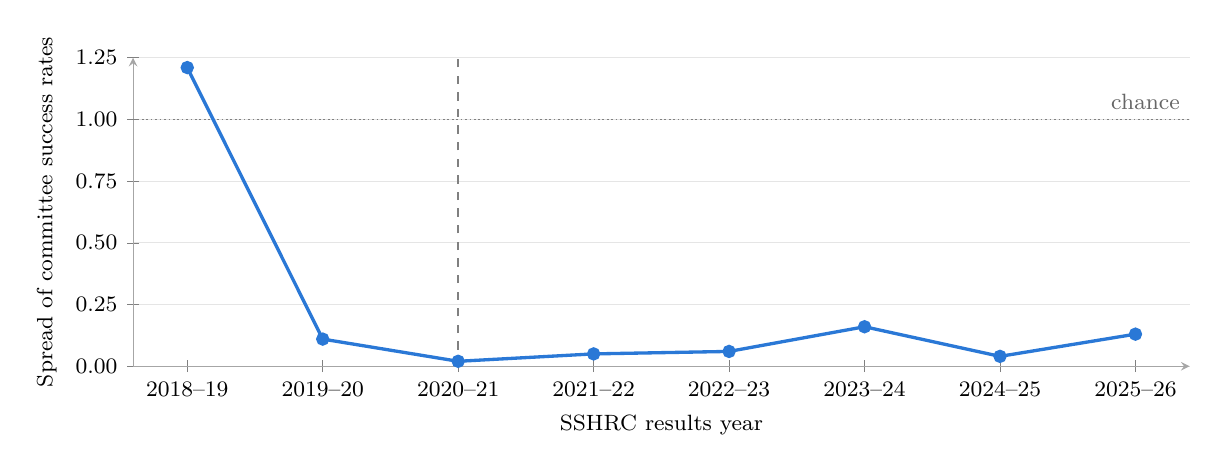
\begin{tikzpicture}
\begin{axis}[
  width=15cm, height=5.5cm,
  xmin=2017.6, xmax=2025.4, ymin=0, ymax=1.25,
  xtick={2018,2019,2020,2021,2022,2023,2024,2025}, xticklabels={2018--19,2019--20,2020--21,2021--22,2022--23,2023--24,2024--25,2025--26},
  axis x line=bottom, axis y line=left, axis line style={gray!70},
  ymajorgrids, grid style={gray!20},
  tick label style={font=\footnotesize}, label style={font=\footnotesize},
  xlabel={SSHRC results year}, ylabel={Spread of committee success rates}, ylabel style={align=center},
  clip=false,
  ytick distance=0.25, yticklabel style={/pgf/number format/.cd, fixed, fixed zerofill, precision=2},
]
\draw[gray, dashed, line width=0.7pt] (axis cs:2020,0) -- (axis cs:2020,1.25);
\addplot[gray, line width=0.6pt, densely dotted, forget plot, domain=2017.6:2025.4, samples=2] {1};
\node[font=\footnotesize, text=gray!80!black, anchor=south east] at (axis cs:2025.4,1) {chance};
\addplot[color=sshrcA, line width=1.2pt, mark=*, mark size=1.8pt] coordinates {(2018.00,1.21) (2019.00,0.11) (2020.00,0.02) (2021.00,0.05) (2022.00,0.06) (2023.00,0.16) (2024.00,0.04) (2025.00,0.13)};
\end{axis}
\end{tikzpicture}
